\chapter{Introduction}

Natural phenomena are a challenging topic in the field of computer graphics.
Actual examples are complex structures which are to be found throughout nature,
such as mountains, trees and water. The latter is especially interesting
because of its highly dynamic form which poses a lot of challenging problems.
Our interest focuses on the geometry of ocean surfaces using
consolidated findings from the oceanographic research community.

\section{Scope and Focus of the Work}

This thesis scope includes the generation of wind driven ocean surfaces, their
animation and illumnation. //FIXME
Since the mathematical models used are not based on fluid dynamics,
convincing interaction between the ocean surface and other objects is beyond the
scope of this work.

wind driven ocean surfaces

Surface geometry, animation, illumination.

\section{Development History}

Work on this thesis started as an extension to \cite{thesis:rost}

\begin{figure}[p]
\begin{center}
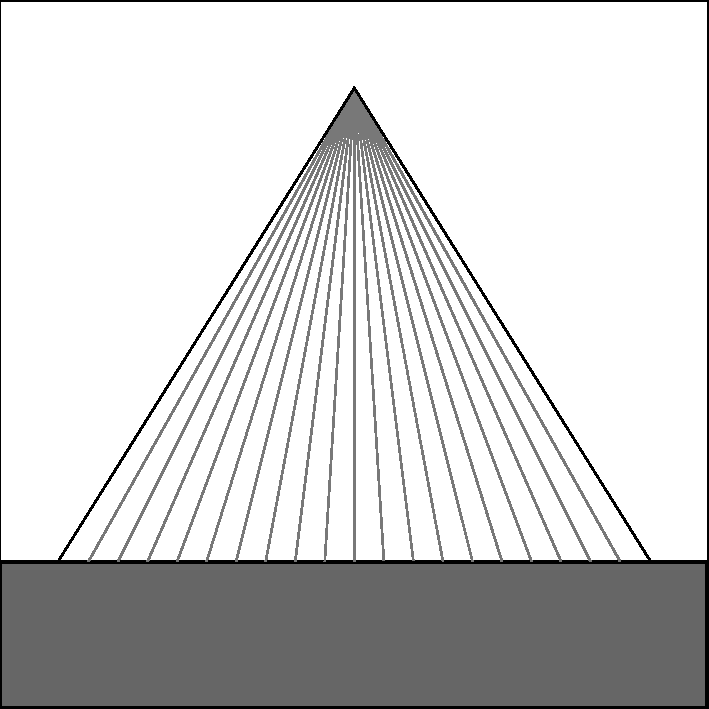
\includegraphics[scale=1.0]{test.pdf}
\end{center}
\end{figure}

\section{Structure of the Thesis}

\begin{itemize}

\item State of the Art
\item Theoretical background
\item Implementation
\item Summary

\end{itemize}

